\documentclass{beamer}
\usetheme{CambridgeUS}
\usepackage{tikz}
\usetikzlibrary{matrix,arrows,fit,positioning, mindmap, trees}

\usepackage[latin1]{inputenc}
\usefonttheme{professionalfonts}
\usepackage{times}
\usepackage{xmpmulti}
\usepackage{animate}
\usepackage{amsmath}
\usepackage{verbatim}
%\usetheme{Boadilla}
%\usecolortheme{crane}
\title[RSA]{Applied Number Theory in Cryptography: RSA}
\subtitle{I Am Curious}
\author{Sebastian Schlesinger}
\institute{Zalando SE}
\date{\today}
\begin{document}
 \begin{frame}
\titlepage
\end{frame}
\begin{frame}
\frametitle{Learning objectives of this presentation}
\begin{itemize}
\item In-depth understanding of RSA with sound mathematical basis
\item Ability to assess constraints w.r.t. selection of various parameters in RSA (e.g. key length, set up of encryption key)
\item Provide formal foundations for further reading in mathematical cryptography
\end{itemize}
\end{frame}
\begin{frame}
\frametitle{Outline}
\tableofcontents
\end{frame}
\section{Foundations of public key cryptography}
%\subsection{Symmetric va. asymmetric ciphers}
 
\begin{frame}
\frametitle{Cryptography: Security Objectives}

\tikzset{rechteck/.style={rectangle, minimum
width=20mm, minimum height=8mm,text centered, draw=black, fill=gray!15, line
width=0.8}}
\tikzset{rechteckfokus/.style={rectangle, minimum
width=20mm, minimum height=8mm,text centered, draw=black, fill=green!15, line
width=0.8}}
\tikzset{rechteckcategory/.style={rectangle, minimum
width=20mm, minimum height=8mm,text centered, draw=black, fill=gray!50, line
width=0.8}}
\begin{center}
\begin{tikzpicture}[node distance=2cm] 

\node (so) [rechteckcategory]{Security Objective};
\node (dummy) [right of=so]{};
\node (int) [rechteckfokus, right of=dummy]{Integrity};
\node (conf) [rechteckfokus, above of=int]{Confidentiality};
\node (ava) [rechteck, below of=int] {Availability};


\draw (so) -- (int);
\draw (so) -- (conf);
\draw (so) -- (ava);


\end{tikzpicture}
\end{center}

\begin{tikzpicture}[node distance=1.5cm] 


\node (target) [rechteckfokus] {Cryptography Target};
\node (dummy) [right of=target] {};
\node (dummy2) [right of=dummy] {};
\node (notarget) [rechteck, right of=dummy2] {No Cryptography Target};




\end{tikzpicture}



\end{frame}

\begin{frame}
\frametitle{The principle of cryptography}

\tikzset{textnode/.style={rectangle, minimum
width=20mm, minimum height=8mm,text centered, draw=black, fill=gray!15, line
width=0.8}}
\tikzset{keynode/.style={rectangle, minimum
width=20mm, minimum height=8mm,text centered, draw=black, fill=green!15, line
width=0.8}}

% \begin{center}
% \begin{tikzpicture}
%   \matrix (m) [matrix of math nodes,row sep=3em,column sep=4em,minimum width=2em]
%   {
%      F_t(x) & F(x) \\
%      A_t & A \\};
%   \path[-stealth]
%     (m-1-1) edge node [left] {$\mathcal{B}_X$} (m-2-1)
%             edge [double] node [below] {$\mathcal{B}_t$} (m-1-2)
%     (m-2-1.east|-m-2-2) edge node [below] {$\mathcal{B}_T$}
%             node [above] {$\exists$} (m-2-2)
%     (m-1-2) edge node [right] {$\mathcal{B}_T$} (m-2-2)
%             edge [dashed,-] (m-2-1);
% \end{tikzpicture}
% \end{center}



\begin{block}{Cryptographic System}
An encryption is a function $enc:K\times P\to C$ from the cartesian product of the set of keys $K$ and the set of plaintexts $P$ to the set cyphertexts $C$. A decryption is a function $dec: K\times C\to P$. A suitable decryption has a key $k'$ such that \[\forall k\in K\forall x\in P: dec(k',enc(k,x))=x\]
Alternative notation for $enc(k,m)$ is $enc_k(m)$.
\end{block}

\end{frame}

\begin{frame}
\frametitle{Desired Properties for Cryptographic Systems}
\begin{enumerate}
\item $enc_k(m)$ must be efficiently computable
\item $dec_{k'}(m)$ must be efficiently computable
\item \textit{Resilience against known ciphertext attack:} Given $c_1,...,c_n\in C$, $dec_{k'}(c_i)$ must not be efficiently computable (without knowledge of $k'$)
\item \textit{Resilience against chosen ciphertext attack:} Given $(m_1,c_1),...,(m_n,c_n)$, $dec_{k'}(c)$ with $c\neq c_i$ should not be efficiently computable
\end{enumerate}
\end{frame}
\begin{frame}
\frametitle{Symmetric and Asymmetric Cryptography}
\begin{block}{Symmetric and Asymmetric Ciphers}
If $k'$ emanates from $k$ efficiently computable, then we speak of a symmetric cipher. Otherwise, it is an asymmetric cipher. 
\end{block}\pause

\tikzset{rechteck/.style={rectangle, minimum
width=20mm, minimum height=8mm,text centered, draw=black, fill=gray!15, line
width=0.8}}
\tikzset{rechteckfokus/.style={rectangle, minimum
width=20mm, minimum height=8mm,text centered, draw=black, fill=green!15, line
width=0.8}}
\tikzset{rechteckcategory/.style={rectangle, minimum
width=20mm, minimum height=8mm,text centered, draw=black, fill=gray!50, line
width=0.8}}
\begin{center}
\begin{tikzpicture}[node distance=4cm] 

\node(pt)[rechteck] {Plaintexts};
\node(dummy)[right of=pt] {};
\node(ct)[rechteck, right of=dummy] {Ciphertexts};

\draw[->] (pt) -- node [above] {$f$ easy to compute} (ct);
\draw[->] (ct) -- node [below] {$f^{-1}$ hard to compute} (pt);
\draw[->] (ct) edge[bend left] node [left, below] {$f^{-1}$ with trapdoor information easy to compute} (pt);

% \draw[->] (-5.5,0) -- (5.5,0) node [below] {$\mathbb{R}$}; \foreach \x in {-5,...,5}
% \draw (\x, 0.1) -- (\x, -0.1) node [below] {\x};


\end{tikzpicture}
\end{center}

\end{frame}
\section{Mathematical background}
\subsection{Basic Structures}
\begin{frame}
\frametitle{Outline}
\tableofcontents
\end{frame}

\begin{frame}
\frametitle{Now let's start with the math}
%\transduration<0-39>{0}
        %\multiinclude[<+->][format=png, graphics={width=\textwidth}]{images/magic}
       \begin{figure}
       \animategraphics[autoplay,controls=none,width=0.5\linewidth]{20}{images/magic-}{0}{39}
       \end{figure}
\end{frame}



\begin{frame}
\frametitle{Groups, Rings, and Fields}
\begin{block}{Groups}
Let $G\neq\emptyset$, $+:G\times G\to G$ a function. $(G,+)$ is said to be an (Abelian) group if and only if the following properties hold.\pause
\begin{itemize}
\item \textit{Associativity:} $\forall x,y,z\in G: (x+y)+z = x + (y+z)$\pause
\item \textit{Commutativity:} $\forall x,y\in G: x+y=y+x$\pause
\item \textit{Neutral Element:} There exists an alement $n$ such that $\forall x\in G: x+n=x$ (denoted as $0$ or $1$ for multiplicative groups)\pause
\item \textit{Inverse Elements:} $\forall x\in G\exists y\in G: x+y=0$. It is called \textit{inverse} of $x$, also denoted as $-x$ or $x^{-1}$ if multiplicatively denoted.
\end{itemize}
\end{block}

\end{frame}

\begin{frame}
\frametitle{Groups, Rings, and Fields}
\begin{block}{Rings with $1$}
Let $R$ be a set with at least two neutral elements $0,1$ w.r.t. the operations $+,\cdot: R\times R\to R$. $(R,+,\cdot)$ is said to be a ring (with $1$) if and only if the following properties hold.
\pause
\begin{itemize}
  \item $(R,+)$ is an Abelian group.\pause
  \item For $(R,\cdot)$ Associativity and Commutativity hold and $1$ is the neutral element.\pause
  \item \textit{Distributivity:} $\forall x,y,z\in R: (x+y)\cdot z=x\cdot z + y\cdot z$.
\end{itemize}
\end{block}

\begin{block}{Example}
An example is the ring of integers $\mathbb{Z}$.
\end{block}

\end{frame}

\begin{frame}
\frametitle{Groups, Rings, and Fields}
\begin{block}{Fields}
Let $F$ be a set with at least two neutral elements $0,1$ w.r.t. the operations $+,\cdot: F\times F\to F$. $(F,+,\cdot)$ is said to be a field if and only if the following properties hold.
\begin{itemize}
  \item $(F,+)$ is an Abelian group.
  \item $(F,\cdot)$ is an Abelian group.
  \item Distributivity holds.
\end{itemize}
\end{block}

\begin{block}{Example}
Examples are the rational numbers $\mathbb{Q}$ and the real numbers $\mathbb{R}$.
\end{block}
\end{frame}
\subsection{Factor Rings}
\begin{frame}
\frametitle{Important relations on integers}
\begin{block}{Divisibility Relation}
For $a,b\in\mathbb{Z}$ we define the divisibility relation $|\subset\mathbb{Z}\times\mathbb{Z}$ as $a|b:\Leftrightarrow\exists m:a\cdot m=b$. It is an order (reflexive, antisymmetric, transitive).
\end{block}
\begin{center}
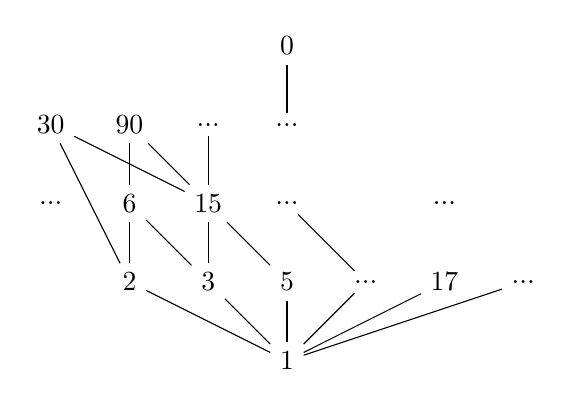
\begin{tikzpicture}[node distance=1cm]
 \node (1)                  {$1$};
 \node (5)  [above of=1]   {$5$};
 \node (3)  [left of=5]  {$3$};
 \node (2)  [left of=3]   {$2$};
 \node (cont1) [right of=5]  {...};
 \node (cont2)  [above of=5]  {...};
 \node (15) [left of=cont2]  {$15$};

 \node (6) [left of=15] {$6$};
 \node (17) [right of=cont1] {$17$};
 \node (cont3) [right of=17] {...};
 \node (cont4) [left of=6] {...};
 \node (cont5) [above of=15] {...};
 %\node (cont6) [above of =cont5] {...};
 \node (cont7) [above of =cont2] {...};
 \node (cont8) [above of =17] {...};
 \node (0)  [above of=cont7] {$0$};
 \node (90) [left of=cont5] {$90$};
  \node (30) [left of=90] {$30$};
 \draw (6) -- (90);
 \draw (15) -- (90);
 \draw (2) -- (30);
 \draw (15) -- (30);
 \draw (15) -- (cont5);
 \draw (1) -- (cont3);
 \draw (1) -- (17);
 \draw (2) -- (6);
 \draw (3) -- (6);
 \draw (1)   -- (5);
 \draw (1)   -- (2);
 \draw (1)   -- (3);
 \draw (1)  -- (cont1);
 \draw (cont1)  -- (cont2);

 \draw (cont7)  -- (0);
 \draw (3)   -- (15);
 \draw (5)   -- (15);
 
\end{tikzpicture}
\end{center}
\end{frame}

\begin{frame}
\frametitle{Important relations on integers}
\begin{block}{Equivalence mod $n$}
For $a,b,n\in\mathbb{Z}$, we define the relation $\equiv\subset\mathbb{Z}\times\mathbb{Z}$ as $a\equiv b\mod n:\Leftrightarrow n|(a-b)$. It is an equivalence relation (reflexive, symmetric, transitive).
\end{block}\pause
An equivalence class for an element $a\in\mathbb{Z}$ is defined as \[[a]:=\{b\in\mathbb{Z}|a\equiv b\mod n\}\] \pause
Elements in $[a]$ yield all the same residue by dividing through $n$. Note that \[\forall x\in\mathbb{Z}\exists \xi,\eta\in\mathbb{Z}: x=\xi\cdot n+\eta\wedge 0\leq\eta <n\] and $\xi,\eta$ are unique.
\end{frame}


\begin{frame}
\frametitle{Factor Ring}
\begin{block}{Factor Ring}
The set of equivalence classes $\mod n$ is defined as \[\mathbb{Z}/n\mathbb{Z}:=\{[a]|a\in\mathbb{Z}\}=\{[0],[1],...,[n-1]\}\] \pause We define operations $+,\cdot$ on it as \[[a]+[b]:=[a+b],[a]\cdot [b]:=[a\cdot b]\] This yields a ring $(\mathbb{Z}/n\mathbb{Z},+,\cdot)$.
\end{block}
\end{frame}
\subsection{Euler's Phi and Lagrange's Theorem}
\begin{frame}
\frametitle{Subgroups and Lagrange's Theorem}

\begin{block}{Lagrange's theorem}
For a group $G$, we call $\#G:=ord(G)$ the order of $G$. For a subgroup $U$ of $G$ always $ord(U)|ord(G)$.
\end{block}\pause

\begin{block}{Orders of elements}
For an element $g\in G$ in a group $G$, the set $\{g^k|k\in\mathbb{Z}\}$ is a subgroup of $G$, its order is denoted $ord(g)$.
\end{block}
\pause
\begin{block}{Corollary to Lagrange's Theorem}
For every element $g\in G$ it holds $g^{ord(G)}=1$.
\end{block}
\end{frame}

\begin{frame}
\frametitle{Ring's multiplikative subgroups and Euler's phi}
\begin{block}{Ring's multiplicative subgroup}
For a ring $R$, we denote the set $R^*:=\{x\in R|\exists y:x\cdot y=1\}$, which is a multiplicative subgroup of $(R,\cdot)$.
\end{block}
\pause
Sufficient condition for $a\in\left(\mathbb{Z}/n\mathbb{Z}\right)^*:$
\[\gcd(a,n)=1\]
\pause
\begin{block}{Examples}
$[1],[3]\in\left(\mathbb{Z}/4\mathbb{Z}\right)^*$: $[1]^{-1}=[1], [3]^{-1}=3, [2]\notin\left(\mathbb{Z}/4\mathbb{Z}\right)^* ([2]\cdot [2]=[0],[2]\cdot [3]=[2])$\\
$1,2,3,4\in\left(\mathbb{Z}/5\mathbb{Z}\right)^*$ 
\end{block}


\end{frame}

\begin{frame}
\frametitle{Euler's phi function}
\begin{block}{Euler's Phi}
We define $\varphi(n):=\#\left(\mathbb{Z}/n\mathbb{Z}\right)^*$.
\end{block}\pause

\begin{block}{Formula for calculating Euler's phi}
For $n=\prod_{p|n}p^{k_p}$, we can calculate \[\varphi (n)=\prod_{p|n}p^{k_p-1}(p-1)=\prod_{p|n}\left(1-\frac{1}{p}\right)\] \pause

\end{block}
Particularly if $n=p\cdot q$, we have \[\varphi(n)=(p-1)\cdot (q-1)\]
\end{frame}
\section{The Algorithm}
\begin{frame}
\frametitle{Outline}
\tableofcontents
\end{frame}

\begin{frame}
\frametitle{Now you no the basics, let's move on to the algorithm...}
\begin{figure}
\animategraphics[autoplay, controls=none,width=0.5\linewidth]{10}{images/algorithm-}{0}{58}
\end{figure}

\end{frame}

\begin{frame}{Encryption}
\begin{block}{Preparation - the public key}
Select two primes $p$ and $q$ and calculate $n=p\cdot q$.\pause

Select $e$ with $1<e<\varphi(n)$ and $\gcd(e,\varphi(n))=1$.\pause

The pair $(n,e)$ is the public key.\pause
\end{block}
For example, $n=5\cdot 11=55$, $\varphi(n)=4\cdot 10=40$, $e=7$.\pause
\begin{block}{Encryption}
A message $m$ with $1<m<n$ is encrypted as follows: \[m^e\equiv c \mod n\] \pause
\end{block}
Say, we encrypt $m=8$. This yields $m^e=8^7\equiv 2\mod 55$, which means $8$ is encrypted by $2$.
\end{frame}

\begin{frame}
\frametitle{Decryption}
\begin{block}{Private Key}
The private key $d$ fulfills \[d\cdot e\equiv 1\mod\varphi (n)\]
\end{block}
$d$ can be obtained via Enhanced Euclidean Algorithm.

\end{frame}

\begin{frame}\frametitle{Enhanced Euclidean Algorithm}
\begin{block}{Purpose of the Enhanced Euclidean Algorithm (EEA)}
The purpose of the EEA is to obtain a representation of the form \[\gcd(a,b)=\xi\cdot a+\eta\cdot b\]
\end{block}\pause

In our example $e=7, \varphi(n)=40$, \pause this yields \[40=5\cdot 7+5, 7=1\cdot 5+2,
5=2\cdot 2+1\] \pause That yields in turn \[\begin{split}\gcd(40,7)=1=5-2\cdot 2=5-2\cdot(7-5)=-2\cdot 7+3\cdot 5\\=-2\cdot 7+3\cdot(40-5\cdot 7)=3\cdot 40-17\cdot 7\end{split}\]\pause
We were looking for $d$ such that $d\cdot e\equiv 1\mod\varphi(n)$. This translates in the example to $d=-17\equiv 23\mod 40$
\end{frame}
\begin{frame}
\frametitle{Decryption Example}
In our example, we have obtained $d=23$.
We had $m=8$ and obtained $c=2$. To decrypt, we calculate \[c^d=2^{23}\equiv 8\mod 55\]
\only\begin{figure}
\animategraphics[autoplay,controls=none,width=0.5\linewidth]{10}{images/gotit-}{0}{54}
\end{figure}
\end{frame}

\subsection{Soundness}
\begin{frame}
\frametitle{Soundness proof: From [complex looking math] it straightforwardly follows...}
\begin{figure}
\animategraphics[autoplay,controls=none,width=0.5\linewidth]{10}{images/complexmath-}{0}{29}
\end{figure}
\end{frame}
\begin{frame}
\frametitle{Soundness for $gcd(m,n)=1$}
If $gcd(m,n)=1$, then $m\in\left(\mathbb{Z}/n\mathbb{Z}\right)^*$. \pause

We know that $\#\left(\mathbb{Z}/n\mathbb{Z}\right)^*=\varphi(n)$ and $\forall x\in \left(\mathbb{Z}/n\mathbb{Z}\right)^*: x^{\varphi(n)}=1$.\pause

Hence, $c^d=\left(m^e\right)^d=m^{e\cdot d}=m^{k\cdot\varphi(n) +1}=m^{k\cdot\varphi(n)}\cdot m=1\cdot m=m$ \\\flushright$\square$
\end{frame}

\begin{frame}
\frametitle{Soundness for $gcd(m,n)\neq 1$}
Let w.l.o.g. $\gcd(m,n)=p$, i.e., $p|m$. \pause

Then $m=p$ or $m=2p$ or $m=p^2$ etc. However, $\gcd(m,q)=1$.\pause

This means $m\in\left(\mathbb{Z}/q\mathbb{Z}\right)^*$, which in turn yields $m^{q-1}=1$, and therefore $m^{k\cdot(q-1)+1}\equiv m\mod q$.\pause

Then $m^{k\cdot (q-1)\cdot (p-1)+1}\equiv m \mod q$, i.e., $m^{k\cdot\varphi(n)+1}\equiv m\mod q$, and of course $m^{k\cdot\varphi(n)+1}\equiv 0\mod q$.\pause

Hence, $m^{k\cdot\varphi(n)+1}-m\equiv 0\mod q$ and $m^{k\cdot\varphi(n)+1}-m\equiv 0\mod p$. \pause

Since $\gcd(p,q)=1$, this yields $m^{k\cdot\varphi(n)+1}-m\equiv 0\mod p\cdot q$.\flushright$\square$
\end{frame}

\begin{frame}
\frametitle{Are you still with me?}
\begin{figure}
\animategraphics[autoplay, loop, controls=none,width=0.5\linewidth]{10}{images/confused-}{0}{49}
\end{figure}


\end{frame}

\section{Security of RSA - Known Attacks (Extract)}
\begin{frame}
\frametitle{Outline}
\tableofcontents
\end{frame}
\begin{frame}
\frametitle{Issues with chosing $p$ and $q$}
Trivial: If $p,q$ too small.\pause

Another issue: If $p,q$ are too close to $\sqrt{n}$: Fermat factorization

\begin{block}{Fermat Factorization}
It is based on the formula $x^2-y^2=(x+y)(x-y)$.

Particularly we consider $n=pq=\left(\frac{p+q}{2}\right)^2-\left(\frac{p-q}{2}\right)^2$.\pause

Let $k$ be the smallest integer so that $k^2>n$, consider $k^2-n$ 

(Note $n=(\sqrt{n})^2)$.\pause

 If this is a square, this yields the factorization $n=(k+h)(k-h)$.\pause

If not, try again with $(k+1)^2-n$, $(k+2)^2-n$ etc.
\end{block}
\begin{block}{Example}
Let $n=6699557$, then $\sqrt{n}\approx 2588.35$. Hence, $k=2589$.\pause

%
$k^2-n=2589^2-6699557=58^2$. Hence, $6699557=2589^2-58^2=(2589+58)(2589-58)=2647\cdot 2531$
\end{block}




\end{frame}

\begin{frame}
\frametitle{Small encryption exponent $e$}
Trivial: If $m<n^{1/e}$, then just take $e-$th root of $c$.\pause

If the same message $m$ is sent encrypted with small exponent $e$, e.g. $3$ to different partners (using different moduli $n_1,n_2,n_3$), then the simultaneous congruence 
\[x\equiv c_1\mod n_1\]
\[x\equiv c_2 \mod n_2\]
\[x\equiv c_3\mod n_3\] can be solved by exploiting Chinese remainder theorem. 

If $m^3<n_1n_2n_3$, this also implies $x=m^3$, which in turn yields the plaintext $m$.

Solution: Salting (Add random bit string to message)
\end{frame}

\begin{frame}
\frametitle{Other attacks}
\begin{itemize} 
  \item Small decryption exponent $d$ ($d<n^{1/4}$): Attackable if $\gcd(p-1,q-1)$ small. Then $d$ can be calculated.
  \item Adaptive chosen cypher text attack due to homomorphic property: $(m_1m_2)^e\equiv m_1^em_2^e\equiv c_1c_2\mod n$.
  \item Coppersmith attacks: Exploit if messages depend linearly on each other, i.e., $m_1=a\cdot m_2+b$
  \item Cycling attacks: For $c=m^e\mod n$, there is a $k$ such that $c^{e^k}\equiv c\mod n$. Hence, $c^{e^{k-1}}\equiv m\mod n$ (like taking $e-$th root of $c$). However, proven to be as hard (and therefore as low-likely as factorization)
  \item Message concealing: If $m^e\equiv m\mod n$ (very small probability).
\end{itemize}
\end{frame}

\begin{frame}
\frametitle{Thank you for your attention}
\begin{figure}
\animategraphics[autoplay, controls=none,width=0.5\linewidth]{20}{images/thanks-}{0}{154}
\end{figure}
\begin{center}
Any Questions?
\end{center}
\end{frame}
\end{document}